\section{Casi d'uso}
    \subsection{Attori dei casi d'uso}
    \subsubsection{Attori primari}
    Gli attori che il gruppo ha ritenuto essere i più adeguati sono:
        \begin{itemize}
            \item \textbf{Utente generico:} si divide in:
                \begin{itemize}
                    \item \textbf{Utente non autenticato:} utente che può navigare nell'e-commerce e può usufruire di alcune funzionalità, come la visualizzazione e la ricerca dei prodotti, che può aggiungere al proprio carrello, la applicazione di filtri e categorie per la ricerca, e infine di potersi autenticare.
                    \item \textbf{Utente autenticato:} un utente autenticato può a sua volta essere:
                        \begin{itemize}
                            \item \textbf{Cliente autenticato:} cliente che ha effettuato il login, può accedere a molte funzionalità, come l'aggiunta di prodotti al carrello, l'acquisto, la visualizzazione della lista degli ordini, la possibilità di contattare il venditore;
                            \item \textbf{Venditore autenticato:} venditore che ha effettuato il login, può accedere alle funzionalità relative all'amministrazione dei prodotti e delle categorie.
                        \end{itemize}
                        \begin{figure}[!ht]
                            \caption{Attori primari}
                            \vspace{5px}
                            
\includegraphics[scale=0.59]{../../../Images/attori}
                            \centering
                        \end{figure}
                \end{itemize}
        \end{itemize}
        \newpage
    \subsection{Elenco dei casi d'uso}
        \textbf{Utilizzo della piattaforma:}
        \begin{figure}[!ht]
            \caption{Casi d'uso che interessano gli utenti}
            \vspace{10px}
            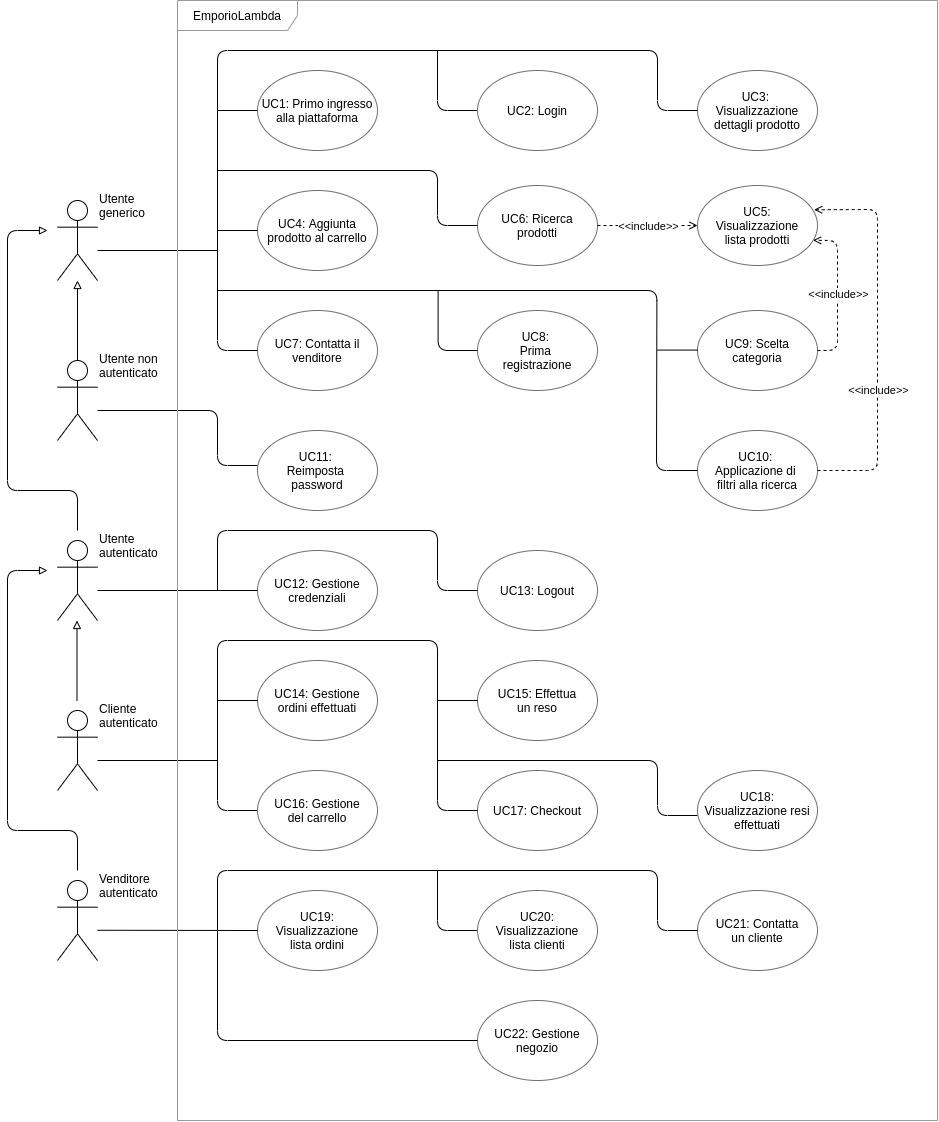
\includegraphics[scale=0.5]{../../../Images/casiUso.png}
            \centering
        \end{figure}
        \subsection{UC1: Primo ingresso alla piattaforma}
        \begin{itemize}
            \item \textbf{Descrizione} L'utente effettua il primo accesso alla piattaforma;
            \item \textbf{Attore Primario} Utente generico;
            \item \textbf{Precondizione} L'utente non sta visualizzando nulla;
            \item \textbf{Postcondizione} L'utente visualizza l'homepage della piattaforma;
            \item \textbf{Scenario Principale} L'utente arriva per la prima volta nell'e-commerce e visualizza l'homepage.
        \end{itemize}
        \subsection{UC2: Login}
        \begin{itemize}
            \item \textbf{Descrizione} Permette l'autenticazione di un utente;
            \item \textbf{Attore Primario} Utente generico;
            \item \textbf{Attore Secondario} Amazon Cognito;
            \item \textbf{Precondizione}L'utente generico non si è ancora autenticato
            \item \textbf{Input} Pressione bottone login;
            \item \textbf{Postcondizione} L'utente è autenticato;
            \item \textbf{Scenario Principale} L'utente entra nella pagina, preme il bottone per il login e viene inderizzato alla pagina di login fornita da \textit{Amazon cognito}.
        \end{itemize}
        \subsection{UC3: visualizzazione dettagli di un prodotto}
        \begin{itemize}
            \item \textbf{Descrizione} L'utente può visualizzare i dettagli di un prodotto di suo interesse;
            \item \textbf{Attore Primario} Utente generico
            \item \textbf{Precondizione} L'utente generico si trova nella pagina della lista dei prodotti;
            \item \textbf{Input} Click sul prodotto (icona, immagine, nome);
            \item \textbf{Postcondizione} L'utente visualizza i dettagli del prodotto d'interesse;
            \item \textbf{Scenario Principale} L'utente all'interno della lista dei prodotti visualizza un prodotto di suo interesse e lo apre e ne visualizza i dettagli.
        \end{itemize}
        \subsection{UC4: Aggiunta di un prodotto al carrello}
        \begin{itemize}
            \item \textbf{Descrizione} L'utente aggiunge al carrello un prodotto che intende acquistare;
            \item \textbf{Attore Primario} Utente generico;
            \item \textbf{Precondizione} L'utente generico di trova nella pagina dettagliata del prodotto;
            \item \textbf{Input} Click sul bottone di aggiunta al carrello;
            \item \textbf{Postcondizione} Il prodotto è stato aggiunto al carrello;
            \item \textbf{Scenario Principale} L'utente una volta deciso il prodotto da acquistare lo aggiunge al proprio carrello tramite l'apposito bottone.
        \end{itemize}
        \subsection{UC5: Ricerca dei prodotti}
        \begin{itemize}
            \item \textbf{Descrizione} L'utente vuole ricercare un prodotto in base ad una parola chiave; 
            \item \textbf{Attore Primario} Utente generico;
            \item \textbf{Precondizione} L'utente si trova in una pagina dedicata alla ricerca; 
            \item \textbf{Input} stringa;
            \item \textbf{Postcondizione} L'utente visualizza i prodotti corrispondenti alla parola chiave;
            \item \textbf{Scenario Principale} Un utente vuole ricercare un prodotto secondo una determinata parola chiave, gli vengo mostrati tutti i risultati della ricerca nella lista dei prodotti;
            \item \textbf{Inclusioni}
            \begin{itemize}
                \item viene visualizzata una pagina con tutti i risultati della ricerca (UC6)
            \end{itemize}
        \end{itemize}
        \subsection{UC6: Visualizzazione della lista dei prodotti}
        \begin{figure}[!ht]
            \caption{Visualizzazione della lista dei prodotti}
            \vspace{10px}
            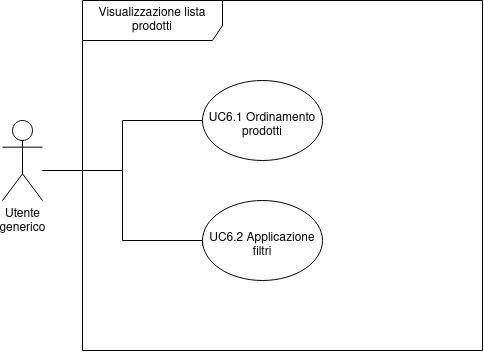
\includegraphics[scale=0.5]{../../../Images/AnalisiRequisiti/UC6.png}
            \centering
        \end{figure}
        \begin{itemize}
            \item \textbf{Descrizione} Un utente visualizza la pagina della lista dei prodotti;
            \item \textbf{Attore Primario} Utente generico;
            \item \textbf{Precondizione} L'utente non sta visualizzando nulla;
            \item \textbf{Postcondizione} L'utente visualizza la pagina con la lista dei prodotti;
            \item \textbf{Scenario Principale} L'utente arriva nella piattaforma e visualizza la lista dei prodotti;
        \end{itemize}
        \subsubsection{UC6.1: Ordinamento prodotti}
        \begin{itemize}
            \item \textbf{Descrizione} L'utente seleziona la modalità in cui visualizzare i file;
            \item \textbf{Attore Primario} Utente generico;
            \item \textbf{Precondizione} L'utente si trova all'interno di una pagina dove l'ordinamento è consentito;
            \item \textbf{Input} selezione parametro scelto
            \item \textbf{Postcondizione} La lista dei prodotti si aggiorna secondo l'ordinamento scelto;
            \item \textbf{Scenario Principale} L'utente si trova all'interno di una pagina che consente l'ordinamento, l'utente seleziona come vuole ordinare i prodotti e la pagina si aggiorna di conseguenza.
        \end{itemize}
        \subsubsection{UC6.2: Applicazione filtri}
        \begin{itemize}
            \item \textbf{Descrizione} L'utente filtra i prodotti in base alle loro caratteristiche;
            \item \textbf{Attore Primario} Utente generico
            \item \textbf{Precondizione} L'utente si trova all'interno di una pagina che consente l'utilizzo di filtri;
            \item \textbf{Input} selezione del filtro desiderato;
            \item \textbf{Postcondizione} La pagina si aggiorna secondo i filtri selezionati;
            \item \textbf{Scenario Principale} L'utente vuole filtrare i prodotti secondo determinate caratteristiche, seleziona questa e la pagina di aggiorna di conseguenza;
        \end{itemize}
        \subsection{UC7: Contatta il venditore}
        \begin{itemize}
            \item \textbf{Descrizione}
            \item \textbf{Attore Primario}
            \item \textbf{Attore Secondario}
            \item \textbf{Precondizione}
            \item \textbf{Input}
            \item \textbf{Postcondizione}
            \item \textbf{Scenario Principale}
            \item \textbf{Inclusioni}
        \end{itemize}
        \subsection{UC8: Prima registrazione}
        \begin{itemize}
            \item \textbf{Descrizione}
            \item \textbf{Attore Primario}
            \item \textbf{Attore Secondario}
            \item \textbf{Precondizione}
            \item \textbf{Input}
            \item \textbf{Postcondizione}
            \item \textbf{Scenario Principale}
            \item \textbf{Inclusioni}
        \end{itemize}
        \subsection{UC9: Scelta della categoria}
        \begin{itemize}
            \item \textbf{Descrizione}
            \item \textbf{Attore Primario}
            \item \textbf{Attore Secondario}
            \item \textbf{Precondizione}
            \item \textbf{Input}
            \item \textbf{Postcondizione}
            \item \textbf{Scenario Principale}
            \item \textbf{Inclusioni}
        \end{itemize}
        \subsection{UC10: Reimposta password (dimenticata)}
        \begin{itemize}
            \item \textbf{Descrizione}
            \item \textbf{Attore Primario}
            \item \textbf{Attore Secondario}
            \item \textbf{Precondizione}
            \item \textbf{Input}
            \item \textbf{Postcondizione}
            \item \textbf{Scenario Principale}
            \item \textbf{Inclusioni}
        \end{itemize}
        \subsection{UC12: Gestione credenziali}
        \subsection{UC13: Logout}
        \subsection{UC14: Gestione degli ordini effettuati}
        \subsection{UC15: Effettua un reso}
        \subsection{UC16: Gestione del carrello}
        \subsection{UC17: Checkout}
        \subsection{UC18: Visualizzazione dei resi effettuati}
        \subsection{UC19: Visualizzazione della lista degli ordini}
        \subsection{UC20: Visualizzazione della lista degli utenti}
        \subsection{UC21: Contatta un cliente}
        \subsection{UC22: Gestione del negozio}

